\documentclass[11pt,a4paper]{article}
\usepackage[margin=2.2cm]{geometry}
\usepackage[T1]{fontenc}
\usepackage[utf8]{inputenc}
\usepackage{lmodern}
\usepackage{microtype}
\usepackage{amsmath,amssymb}
\usepackage{booktabs}
\usepackage{array}
\usepackage{enumitem}
\usepackage{caption}
\usepackage{subcaption}
\usepackage{xcolor}
\usepackage{tikz}
\usetikzlibrary{arrows.meta,positioning,calc,fit,backgrounds}
\usepackage{pgfplots}
\pgfplotsset{compat=1.17}
\usepackage[hidelinks]{hyperref}

\definecolor{cours}{HTML}{3B6EA8}
\definecolor{cludvig}{HTML}{E08A2E}
\definecolor{coccam}{HTML}{3D9A6B}
\definecolor{cgrey}{HTML}{777777}
\newcommand{\hit}{\textcolor{coccam}{$\bullet$}}
\newcommand{\miss}{\textcolor{cgrey}{$\circ$}}
\newcommand{\code}[1]{\texttt{\small #1}}
\makeatletter\newcommand{\inputtable}[1]{\@@input #1 }\makeatother

\title{\textbf{Full pipelines of LUDVIG and Occam's LGS}\\[2pt]
\large The papers' own feature extraction, lift and refinement on backroom and flightroom}
\author{Radiance FYP --- semantic embedding\\ \small intellisense08 (RTX 2080, 8\,GB), runs 13--14 October 2026, report 16 October 2026}
\date{}

\begin{document}
\maketitle

\begin{abstract}
\noindent The controlled comparison of 13 October swapped only the lift and found it does not matter: LUDVIG's lift equals
ours, and Occam's centre-pixel lift is within $\pm2$ queries. Here we run each paper's \emph{whole} pipeline with the
authors' code. For LUDVIG that is DINOv2 ViT-g/14 features reduced by PCA to 40 dimensions, its own CLIP crop pyramid,
and its DINOv2 graph diffusion of CLIP relevancy. For Occam's LGS it is LangSplat's language features: SAM ViT-H masks at
three granularities, one OpenCLIP embedding per mask, lifted per level. Our query and evaluator score both, unchanged.
\textbf{Occam's full pipeline is the best configuration we have measured: 25/29 objects found with only 1 of 6 absent
objects firing}, at every floor from 0.52 to 0.55. The best earlier design reached 22/29 at the default floor
and 19/29 at one false positive. \textbf{LUDVIG's full pipeline does not improve on our lift} (19/29; 18/29 with its
diffusion). The gain comes from region-level CLIP features on high-quality SAM masks, not from the lift. It costs about
5 GPU-hours of feature extraction per scene.
\end{abstract}

\tableofcontents
\bigskip

\section{Key findings}
\begin{enumerate}[leftmargin=*,itemsep=2pt]
  \item \textbf{Occam's full pipeline: 25/29, 1/6 false positives.} Backroom 12/13 and flightroom 13/16 at the default floor
        0.55. AUROC of peak relevancy, positives against absent objects, is 0.92 on backroom and 1.00 on flightroom. Against
        our default lift (A, 22/29) it gains \emph{swivel chair}, \emph{camera tripod} and \emph{hose reel} and loses
        nothing. Camera tripod had been found once before (Occam's lift on the A teachers, 13 Oct) and swivel chair only with
        DINO diffusion on A; no earlier configuration found both. Development set: 5/5.
  \item \textbf{It holds at equal false positives.} The floor sweep gives 25/29 at every false-positive budget from 1 to 5
        (one false positive at floors 0.52--0.55, 24/29 at 0.575). Every other design gives 19/29 at one false positive and at most 24/29 at five
        (\S\ref{sec:sweep}). This is not a floor effect.
  \item \textbf{Choosing the level per query matters.} The same table scored without the per-query choice among the three
        SAM levels (flat) gives 23/29 at one false positive. Choosing the level whose relevancy peaks highest, as
        LangSplat's evaluation does, adds two.
  \item \textbf{LUDVIG's full pipeline: 19/29 (L-C), 19/29 with our DINO step (L-CD), 18/29 with its own diffusion (L-CL).}
        Its CLIP peaks run 0.01--0.03 below ours, which costs one object at the fixed floor and removes one false
        positive. Its diffusion only reshapes which Gaussians are selected once an object clears the floor; it cannot
        recover objects whose relevancy never reaches the floor, which are most of our misses. Once it sent the
        flightroom garden cart to a region 16\,m away.
  \item \textbf{Cost.} LangSplat's SAM ViT-H extraction took 5.1\,h (backroom, 270 images at 1080p) and 4.7\,h (flightroom,
        450 at 720p) on the RTX 2080. Our teacher extraction takes 31--53\,min. Occam's lift then needs 28--34\,s.
        LUDVIG's features took 29 / 37\,min and its diffusion 2--4\,min per scene.
\end{enumerate}

\section{What was run}
\subsection{The two pipelines}

\begin{figure}[h]
\centering
\resizebox{\linewidth}{!}{%
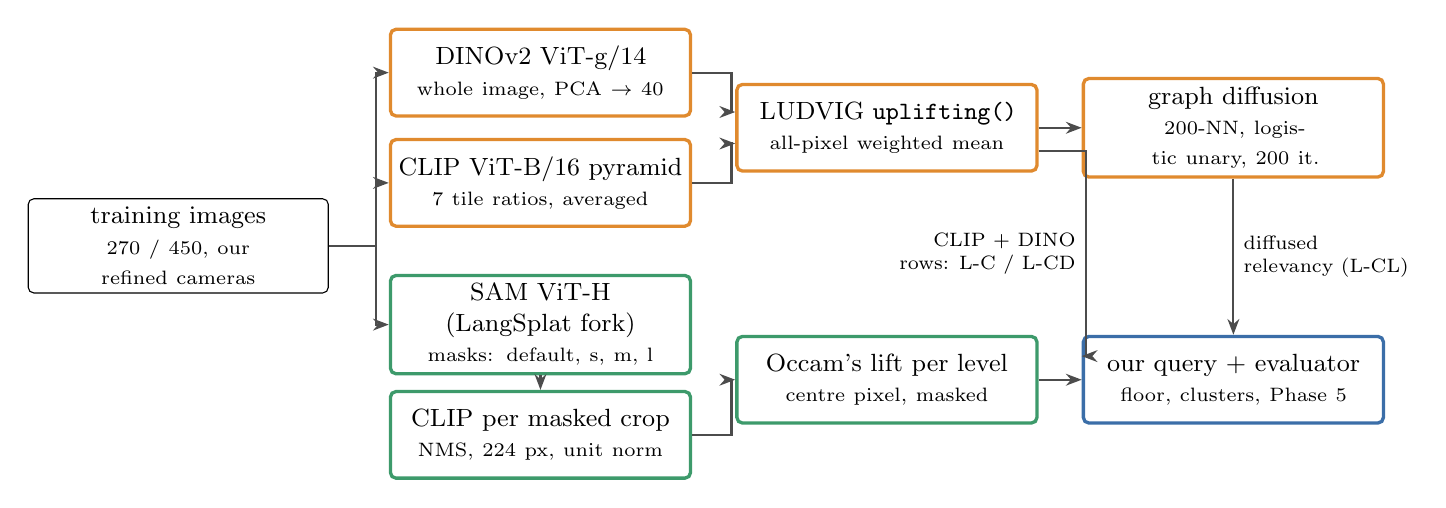
\begin{tikzpicture}[font=\small,
  box/.style={draw, rounded corners=2pt, align=center, minimum height=11mm, text width=36mm, inner sep=3pt, fill=white},
  lud/.style={box, draw=cludvig, very thick}, occ/.style={box, draw=coccam, very thick}, ours/.style={box, draw=cours, very thick},
  arr/.style={-{Stealth[length=2mm]}, thick, draw=black!70}]
  \node[box] (img) at (0,-1.6) {training images\\\scriptsize 270 / 450, our refined cameras};
  \node[lud] (dino) at (4.6, 0.6) {DINOv2 ViT-g/14\\\scriptsize whole image, PCA $\to$ 40};
  \node[lud] (clip) at (4.6,-0.8) {CLIP ViT-B/16 pyramid\\\scriptsize 7 tile ratios, averaged};
  \node[lud] (up)   at (9.0,-0.1) {LUDVIG \code{uplifting()}\\\scriptsize all-pixel weighted mean};
  \node[lud] (dif)  at (13.4,-0.1) {graph diffusion\\\scriptsize 200-NN, logistic unary, 200 it.};
  \node[occ] (sam)  at (4.6,-2.6) {SAM ViT-H (LangSplat fork)\\\scriptsize masks: default, s, m, l};
  \node[occ] (lsf)  at (4.6,-4.0) {CLIP per masked crop\\\scriptsize NMS, 224 px, unit norm};
  \node[occ] (olift) at (9.0,-3.3) {Occam's lift per level\\\scriptsize centre pixel, masked};
  \node[ours] (q)   at (13.4,-3.3) {our query + evaluator\\\scriptsize floor, clusters, Phase 5};
  \draw[arr] (img.east) -- ++(0.6,0) |- (dino.west);
  \draw[arr] (img.east) -- ++(0.6,0) |- (clip.west);
  \draw[arr] (img.east) -- ++(0.6,0) |- (sam.west);
  \draw[arr] (sam) -- (lsf);
  \draw[arr] (dino.east) -- ++(0.5,0) |- ([yshift=2mm]up.west);
  \draw[arr] (clip.east) -- ++(0.5,0) |- ([yshift=-2mm]up.west);
  \draw[arr] (up) -- (dif);
  \draw[arr] (lsf.east) -- ++(0.5,0) |- (olift.west);
  \draw[arr] (olift) -- (q);
  \draw[arr] (dif) -- node[right, font=\scriptsize, align=left] {diffused\\relevancy (L-CL)} (q);
  \draw[arr] ([yshift=-3mm]up.east) -- ++(0.6,0) |- ([yshift=3mm]q.west) node[pos=0.25, left, font=\scriptsize, align=right] {CLIP + DINO\\rows: L-C / L-CD};
\end{tikzpicture}}
\caption{The two full pipelines (orange: LUDVIG; green: Occam's LGS with LangSplat's features; all the authors' code) and
our scoring (blue). Both start from the same images and refined cameras.}
\label{fig:pipes}
\end{figure}

\paragraph{LUDVIG} (branch \code{semantic/LUDVIG}; \code{ludvig\_full.py}, \code{ludvig\_diffuse.py}). It follows
LUDVIG's LERF configuration (\code{lerf\_dinov2.yaml}, \code{lerf\_clip.yaml}, \code{lerf\_eval.yaml}). Images are read by
its loader (longest side 1600\,px) and renders use the same size. DINOv2 runs on the whole image; tokens are
standardised per channel and projected to 40 PCA components fitted on 500k random tokens (62\,\% of the variance on both
scenes). CLIP is its 7-tile-ratio sliding window (0.05--0.5), averaged and normalised. Both are lifted with its
\code{uplifting()}. The diffusion is its \code{GraphDiffusionCLIP} over all query texts of a scene at once (21 backroom,
19 flightroom), as its LERF script runs all prompts of a scene: a 200-nearest-neighbour graph, an RBF on DINO distance
scaled by the median, a logistic-regression unary term seeded by Otsu, and 200 power iterations.

\paragraph{Occam's LGS} (branch \code{semantic/LGS}; \code{langsplat\_features.py}, \code{occam\_lift.py --langsplat}).
Occam's paper lifts LangSplat's feature maps, so they are produced with LangSplat's \code{preprocess.py} and its SAM fork.
That means SAM ViT-H automatic masks (32 points per side, one crop layer, IoU 0.7, stability 0.85, min region 100\,px),
returned at four granularities. Masks are filtered by LangSplat's mask NMS (IoU 0.8, score 0.7, inner 0.5), each mask's
bounding box on black is padded square at 224\,px, and one OpenCLIP ViT-B/16 embedding is taken per mask. Occam's
accumulation then lifts levels s, m, l (its \code{feature\_level} 1--3) separately at the seg-map resolution, skipping
pixels no mask covers, as its \code{get\_language\_feature} does. The three levels go into the table's scale groups, so our
query picks the level per query, which is LangSplat's evaluation rule. After NMS an image keeps a median of 544 masks over
its four levels on backroom and 263 on flightroom.

\subsection{Turning the papers' outputs into a 3D goal}
Neither paper outputs a 3D goal: both evaluate 2D masks or argmax pixels. Everything after the per-Gaussian features is
our query: LERF relevancy, floor 0.55, relative threshold, 0.1\,m voxel clusters of $\geq15$ Gaussians, and approach
point. For LUDVIG's diffusion we add one variant, \textbf{L-CL}: the raw CLIP peak must clear the floor, as in every
variant, and the Gaussians are then those whose diffused relevancy, normalised by its maximum, exceeds an Otsu
threshold over its positive values. That is LUDVIG's own segmentation rule (\code{evaluation\_diffusion: cutoff 0}),
applied in 3D instead of 2D. Our Otsu matches \code{skimage.filters.threshold\_otsu} exactly (unit test).

\subsection{Changes needed on an 8\,GB GPU}
The authors ran on 48\,GB GPUs. Every change below alters only memory use or speed, never the numbers, and each is
documented in the runner's header.
\begin{itemize}[leftmargin=*,itemsep=1pt]
  \item \textbf{LUDVIG.} PCA tokens are kept in host RAM (12\,GB) instead of on the GPU. Each CLIP scale is upsampled
        and added in 64-channel chunks. Crops are encoded in batches of 128. Each CLIP map is released before the next
        is built, because \code{uplifting()}'s loop variable otherwise kept two 2.75\,GB maps alive. DINO and CLIP run as
        separate processes. In the diffusion, the $N\times201\times40$ distance tensor (17\,GB) is computed in chunks,
        and the 214M-entry sparse power iterations run on the CPU.
  \item \textbf{LangSplat.} One image per \code{create()} call. SAM decodes 16 prompts per batch instead of 64; each point
        is decoded independently. The mask NMS is vectorised: a pairwise-intersection matrix summed over pixel chunks,
        with upstream's rules applied elementwise. Upstream compares all mask pairs in a Python loop, which is
        infeasible at hundreds of masks per level (647 on one backroom image). On real masks it keeps exactly the same masks as upstream on all
        ten level sets checked (\code{raw/logs/test\_langsplat\_nms.log}) and is 10--40$\times$ faster.
  \item \textbf{Occam's lift.} LangSplat feature maps are held in fp16, the precision LangSplat stores them in.
\end{itemize}

\subsection{Properties of the released code, kept as they are}
\begin{itemize}[leftmargin=*,itemsep=1pt]
  \item \textbf{LUDVIG drops the DINOv2 register tokens.} Its vendored ViT has no register tokens, and the checkpoint is
        loaded with \code{strict=False}, so the \code{reg4} checkpoint's \code{register\_tokens} are silently discarded
        (the run log lists the skipped key). The paper's "ViT-g with registers" therefore runs without them.
  \item \textbf{LUDVIG's \code{prune\_gaussians: 600000}} keeps every Gaussian of a scene with fewer than 600k, but
        re-sorts them by weight. We skip it to keep checkpoint order; it does not change the features.
  \item \textbf{LUDVIG's lifting kernel} counts each blend weight once per channel; this has no effect after normalisation
        (13 Oct report).
\end{itemize}

\section{Results on the Phase 5 sets}\label{sec:results}
\begin{table}[h]
\centering\small
\caption{Phase 5 sets (29 positives, 6 absent objects; query settings unchanged since Phase 1). Totals over both
scenes, then per scene: hits, median localisation error (m), AUROC of peak relevancy. L-C: CLIP relevancy; L-CD: plus
our DINO diffusion and split; L-CL: LUDVIG's graph diffusion.}
\label{tab:summary}
\setlength{\tabcolsep}{3.5pt}
\begin{tabular}{llcc ccc ccc}
\toprule
& & & & \multicolumn{3}{c}{backroom} & \multicolumn{3}{c}{flightroom}\\
\cmidrule(lr){5-7}\cmidrule(lr){8-10}
Configuration & mode & hits & FP & hits & err & AUROC & hits & err & AUROC\\
\midrule
\inputtable{tables/summary.tex}
\bottomrule
\end{tabular}
\end{table}

\begin{figure}[h]
\centering
\begin{tikzpicture}
\begin{axis}[ybar, width=\linewidth, height=5.6cm, bar width=7pt, ymin=14, ymax=27,
  symbolic x coords={Ours-Old,Ours-A,B2,LUDVIG-ctrl,LUDVIG-full,Occam-ctrl,Occam-full}, xtick=data,
  x tick label style={font=\scriptsize}, enlarge x limits=0.08, ylabel={top-1 hits (of 29)},
  legend style={at={(0.5,1.03)}, anchor=south, legend columns=3, font=\scriptsize},
  nodes near coords, every node near coord/.append style={font=\tiny}, grid=major, grid style={gray!20},
  unbounded coords=discard]
  \addplot[fill=cours!70, draw=cours] table[x=config, y=LC, col sep=comma] {data/bars.csv};
  \addplot[fill=black!25, draw=black!60] table[x=config, y=LCD, col sep=comma] {data/bars.csv};
  \addplot[fill=cludvig!60, draw=cludvig] table[x=config, y=LCL, col sep=comma] {data/bars.csv};
  \legend{L-C, L-CD, L-CL (LUDVIG diffusion)}
\end{axis}
\end{tikzpicture}
\caption{Top-1 hits over both scenes. "ctrl" = the 13 Oct controlled runs (the paper's lift on our teachers). "full"
= the paper's whole pipeline.}
\label{fig:bars}
\end{figure}

\begin{table}[p]
\centering\small
\caption{Per-query outcome (\hit\ hit, \miss\ miss). Bold queries differ between configurations.}
\label{tab:perquery}
\begin{tabular}{l cccccc}
\toprule
& Ours A & B2 & LUDVIG full & LUDVIG full & Occam lift & Occam full\\
Query & L-C & L-C & L-C & L-CL & A, L-C & L-C\\
\inputtable{tables/per_query.tex}
\bottomrule
\end{tabular}
\end{table}

\paragraph{Reading.}
\begin{itemize}[leftmargin=*,itemsep=2pt]
  \item \textbf{Occam's full pipeline} misses only \emph{white bucket} (wrong object, 1.8\,m away) in backroom. In
        flightroom it misses \emph{keyboard} (peak 0.556, no candidate), \emph{floor lamp} and \emph{drone gate} (both 0.87--0.97\,m off,
        "bad position"). These three and the white bucket are missed by every configuration in this report; floor lamp and keyboard are CLIP
        recognition limits (SEMANTICS.md \S14). Its peaks for the occluded chairs rise sharply (flightroom armchair 0.708
        vs 0.582 for A; upholstered chair 0.654 vs 0.553): a SAM mask isolates the chair from the whiteboard in front of
        it, and a crop embedding of the chair alone matches the text far better than a fixed-size crop.
  \item \textbf{Absent objects.} Only backroom's \emph{ceiling fan} fires (peak 0.647), which every design has found at
        every floor and is probably a real look-alike in the room (HANDOVER \S2.5). Flightroom's \emph{recycling bin},
        which fires for A, stays below the floor (0.533).
  \item \textbf{Localisation error is higher} (median 0.27 / 0.30\,m vs 0.21 / 0.25\,m for A). Region features spread
        evenly over a whole object, including its far side, so the candidate centroid sits less often on the visible face
        that the annotation marks. All hits are within the 0.75\,m hit radius by definition, and the approach point
        uses a 1\,m standoff.
  \item \textbf{Our B2} (SAM ViT-B, levels by mask area, pyramid features where no mask covers a pixel) reached 21/29.
        LangSplat's recipe differs in four ways: SAM ViT-H with a second crop layer; SAM's own granularities instead of
        area bins; mask NMS; and unsegmented pixels \emph{skipped} rather than filled with pyramid features. Which of these
        carries the gain is not separated by this experiment.
  \item \textbf{LUDVIG full} misses the same objects as our Old lift, plus \emph{office chair} (peak 0.534, just under the
        floor). L-CL then loses \emph{garden cart} in flightroom: diffusion carried its weight to Gaussians 16\,m away,
        outside the room, which looks like seeds on floaters.
\end{itemize}

\subsection{Development set}
\begin{table}[h]
\centering\small
\caption{Development set (5 backroom queries, \code{phase1\_gate}).}
\label{tab:dev}
\begin{tabular}{lccl}
\toprule
Configuration & hits & err (m) & missed\\
\midrule
\inputtable{tables/dev.tex}
\bottomrule
\end{tabular}
\end{table}

\section{Floor sweep}\label{sec:sweep}
\begin{figure}[h]
\centering
\begin{subfigure}{0.49\linewidth}
\begin{tikzpicture}
\begin{axis}[width=\linewidth, height=5.4cm, xlabel={relevancy floor}, ylabel={top-1 hits (of 29)}, ymin=12, ymax=27,
  legend style={font=\tiny, at={(0.5,-0.3)}, anchor=north, legend columns=2}, grid=major, grid style={gray!20}]
  \addplot[cours, thick, mark=*, mark size=1.2pt] table[x=floor, y=Old_hits, col sep=comma] {data/floor_sweep.csv};
  \addplot[cours, thick, dashed, mark=square*, mark size=1.2pt] table[x=floor, y=A_hits, col sep=comma] {data/floor_sweep.csv};
  \addplot[cludvig, thick, mark=triangle*, mark size=1.4pt] table[x=floor, y=LUDVIGfull_hits, col sep=comma] {data/floor_sweep.csv};
  \addplot[coccam, very thick, mark=diamond*, mark size=1.6pt] table[x=floor, y=Occamfull_hits, col sep=comma] {data/floor_sweep.csv};
  \addplot[coccam, thick, dashed, mark=o, mark size=1.4pt] table[x=floor, y=Occamfullflat_hits, col sep=comma] {data/floor_sweep.csv};
  \legend{Ours Old, Ours A, LUDVIG full, Occam's full, Occam's full flat}
\end{axis}
\end{tikzpicture}
\caption{Hits vs floor.}
\end{subfigure}\hfill
\begin{subfigure}{0.49\linewidth}
\begin{tikzpicture}
\begin{axis}[width=\linewidth, height=5.4cm, xlabel={absent objects with a candidate (of 6)}, ylabel={top-1 hits (of 29)},
  ymin=12, ymax=27, xmin=-0.5, xmax=6.5, legend style={font=\tiny, at={(0.5,-0.3)}, anchor=north, legend columns=2},
  grid=major, grid style={gray!20}]
  \addplot[cours, only marks, mark=*] table[x=Old_fp, y=Old_hits, col sep=comma] {data/floor_sweep.csv};
  \addplot[cours, only marks, mark=square] table[x=A_fp, y=A_hits, col sep=comma] {data/floor_sweep.csv};
  \addplot[cludvig, only marks, mark=triangle*] table[x=LUDVIGfull_fp, y=LUDVIGfull_hits, col sep=comma] {data/floor_sweep.csv};
  \addplot[coccam, only marks, mark=diamond*, mark size=3pt] table[x=Occamfull_fp, y=Occamfull_hits, col sep=comma] {data/floor_sweep.csv};
  \addplot[coccam, only marks, mark=o, mark size=2.5pt] table[x=Occamfullflat_fp, y=Occamfullflat_hits, col sep=comma] {data/floor_sweep.csv};
  \legend{Ours Old, Ours A, LUDVIG full, Occam's full, Occam's full flat}
\end{axis}
\end{tikzpicture}
\caption{Hits vs false positives (one point per floor).}
\end{subfigure}
\caption{Relevancy-floor sweep, floors 0.46--0.60, both scenes combined. Old and A are the 13 Oct sweep.}
\label{fig:sweep}
\end{figure}

\begin{table}[h]
\centering\small
\caption{Best hits (of 29) over the swept floors with at most $k$ absent objects firing (post-hoc on the evaluation
sets, optimistic for every row alike).}
\label{tab:envelope}
\begin{tabular}{lccccc}
\toprule
$k$ absent objects with a candidate & 1 & 2 & 3 & 4 & 5\\
\midrule
\inputtable{tables/envelope.tex}
\bottomrule
\end{tabular}
\end{table}

\paragraph{Reading.} Occam's full pipeline holds 25/29 with one false positive over floors 0.52--0.55 (backroom
11--12/13, flightroom 13--14/16 with no absent object firing); it drops to 24/29 at 0.575 and adds backroom's bicycle at 0.50--0.51. Its curve is flat where every other design trades hits
for false positives. At floors 0.50--0.525 it finds 14/16 in flightroom, with no false positive there. The flat
variant without level choice sits two below throughout. LUDVIG's full pipeline tracks our Old and A curves within one
query. On 29 queries the 25 vs 22 at the default floor is three gains and no losses (exact sign test $p=0.25$), so it is
not formally significant. But it comes with fewer false positives, higher AUROC and a stable curve, which a lucky floor
would not give.

\section{Cost}\label{sec:cost}
\begin{table}[h]
\centering\small
\caption{Cost on the RTX 2080. "Features + lift": for ours and B2 the lift alone (teacher extraction, shared, is
another 31--53\,min per scene, B2's 41--47\,min). For LUDVIG full, its own feature extraction and lift. For Occam's
full, LangSplat's extraction plus Occam's lift. Seen = Gaussians with weight $>0$. Table size in GB.}
\label{tab:cost}
\resizebox{\linewidth}{!}{%
\begin{tabular}{l cccc cccc}
\toprule
& \multicolumn{4}{c}{backroom (532k Gaussians, 270 views)} & \multicolumn{4}{c}{flightroom (380k, 450 views)}\\
\cmidrule(lr){2-5}\cmidrule(lr){6-9}
Configuration & feat.+lift (min) & diffusion (min) & seen (\%) & GB & feat.+lift (min) & diffusion (min) & seen (\%) & GB\\
\midrule
\inputtable{tables/cost.tex}
\bottomrule
\end{tabular}}
\end{table}

\noindent LangSplat's extraction is dominated by SAM ViT-H's automatic mask generator: 5 crops $\times$ 1,024 prompts per
image, about 70--100\,s per 1080p image on the 2080. This is a one-off per scene, run offline like our teachers. After
that, Occam's lift (30\,s) and queries (2--3\,s, three levels) are cheap. On the RTX 5060 Ti the extraction should be
several times faster.

\section{Discussion and next steps}
\paragraph{What the two experiments show together.} On 13 Oct, swapping only the lift changed nothing: all-pixel and
centre-pixel lifts are equivalent on our scenes. Here, swapping the \emph{2D features} changes a lot. Region-level CLIP on
SAM ViT-H masks, chosen per query among three granularities, finds 25/29 against 22/29 and rejects absent objects better.
A larger DINO model with LUDVIG's diffusion does not help, because our misses are recognition and isolation failures
before any 3D step. The Phase 5 diagnosis (SEMANTICS.md \S14) said the loss happens in 2D, and this is the clearest
confirmation: the best 2D features win, whatever lifts them.

\paragraph{Caveats.} 29 positives and 6 absent objects over two scenes; the improvement is +3 queries. The
evaluation positions were placed by Claude from photos, independently of every method. LangSplat's features were run
exactly once (SAM's automatic generator is deterministic given the image). Localisation error is about 0.05\,m higher.

\paragraph{For \code{semantic/new}.}
\begin{enumerate}[leftmargin=*,itemsep=2pt]
  \item \textbf{Adopt region-level features as the base}: SAM masks at several granularities, one CLIP embedding per
        masked crop, lifted per level, with the level chosen per query. This is the strongest design measured.
  \item \textbf{Separate what makes LangSplat's recipe better than our B2}: SAM ViT-H vs ViT-B, SAM granularities vs
        area bins, skipping vs filling unsegmented pixels, mask NMS. All four can be tested by re-lifting cheaply (30\,s)
        once masks are cached. The skip-vs-fill choice can be tested on the existing LangSplat cache today.
  \item \textbf{Reduce the extraction cost}: SAM 2 or an efficient SAM, fewer prompt points, or no crop layer, each
        measured against the 25/29 reference.
  \item \textbf{Fix the localisation offset}: use the masks themselves to anchor the candidate on the visible surface, or
        weight the centroid by view-facing Gaussians.
  \item \textbf{Remaining misses} (keyboard, floor lamp, drone gate, white bucket) need recognition beyond CLIP ViT-B/16
        crops, for example a re-ranker on the top candidates (HANDOVER \S2.2 item 3).
\end{enumerate}

\section{Reproduction}
{\scriptsize
\begin{verbatim}
# semantic/LUDVIG (worktree ~/Radiance/rese-ludvig)
source semantics/baselines/env.sh ludvig
python semantics/baselines/ludvig_full.py --scene backroom --only dino
python semantics/baselines/ludvig_full.py --scene backroom --only clip
python semantics/baselines/ludvig_diffuse.py --scene backroom
source ~/Radiance/figs/figs_env.sh
python figs/semantic_pipeline.py --scene backroom --backend lift --table-suffix _ludvigfull \
       --clip-mode pyramid --only export
python semantics/baselines/import_diffused.py --scene backroom
python -m radiance_semantics.evaluate --scene backroom \
       --variants L-C@ludvigfull L-CD@ludvigfull L-CL@ludvigfull
# semantic/LGS
source semantics/baselines/env.sh occamlgs
python semantics/baselines/langsplat_features.py --scene backroom            # ~5 h on the RTX 2080
python semantics/baselines/occam_lift.py --scene backroom --langsplat ~/Radiance/third_party/langsplat_features \
       --suffix _occamfull
source ~/Radiance/figs/figs_env.sh
python figs/semantic_pipeline.py --scene backroom --backend lift --table-suffix _occamfull \
       --clip-mode scales --only export
python -m radiance_semantics.evaluate --scene backroom --variants L-C@occamfull
\end{verbatim}
}
\noindent Raw results are in \code{../raw/} (evaluator JSONs for Phase 5 and the development set, lift statistics,
LangSplat metadata, floor sweep, logs including the NMS equivalence check), derived CSVs in \code{../csv/}, and
\code{../scripts/collect.py}, \code{make\_tables.py} regenerate them. The LangSplat feature cache (15\,GB) is at
\code{\textasciitilde/Radiance/third\_party/langsplat\_features/}.

\end{document}
